\section*{Random}

Unconstrained optimization:

\begin{minipage}{\columnwidth}
    \centering
    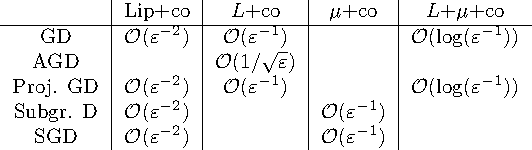
\includegraphics[width=\columnwidth]{../assets/unconstrained-cvg-table/unconstrained-cvg-table.pdf}
\end{minipage}

LMO: Let $X := \text{conv}(\mathcal{A})$, then:

\begin{minipage}{\columnwidth}
    \centering
    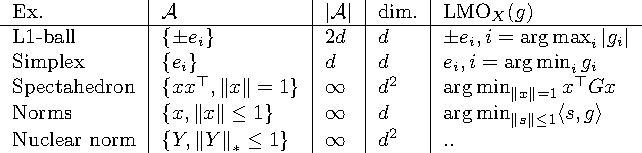
\includegraphics[width=\columnwidth]{../assets/lmo-table/lmo-table.pdf}
\end{minipage}

% Todo table for subgradient descent
Performance of AGD vs Subgr. D:

\begin{minipage}{0.8\columnwidth}
    \centering
    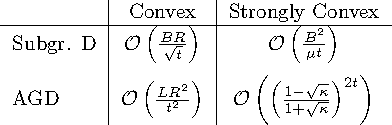
\includegraphics[width=\columnwidth]{../assets/non-smooth-subgr-table/non-smooth-subgr-table.pdf}
\end{minipage}

$\rightarrow$ Subgr. D is always slower, even in sc case only sublinear cvg.

Complexity for SGD:

\begin{minipage}{\columnwidth}
    \centering
    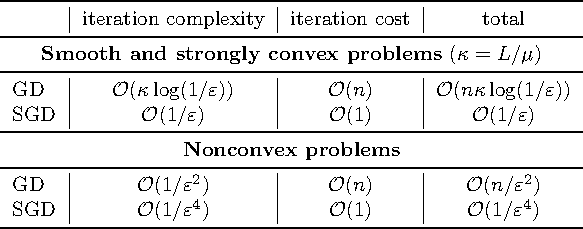
\includegraphics[width=\columnwidth]{../assets/sgd-table/sgd-table.pdf}
\end{minipage}

\textbf{Vanilla Analysis (GD \& Proj. GD):}
\begin{enumerate}
\item Use 1oc: $f(y) \geq f(x) + \nabla f(x)^\top (y-x)$
\item Set $y=x^*$, $x=x_t$: $\varepsilon_t \leq \nabla f(x_t)^\top (x_t - x^*)$
\item Use update rule: $x_t - x^* = (z_{t+1} - x^*) + \gamma \nabla f(x_t)$
    \\ where $z_{t+1} = x_{t+1}$ for GD, $z_{t+1} = y_{t+1}$ for Proj. GD
\item Apply cosine theorem: $2v^\top w = \lVert v \rVert^2 + \lVert w \rVert^2 - \lVert v-w \rVert^2$
\item For Proj. GD: Use projection property $\lVert x_{t+1} - x^* \rVert^2 \leq \lVert y_{t+1} - x^* \rVert^2$
\item Sum over $t$, telescope: $\sum_{t=0}^{T-1} \varepsilon_t \leq \frac{\gamma}{2} \sum_{t=0}^{T-1} \lVert \nabla f(x_t) \rVert^2 + \frac{1}{2\gamma} \lVert x_0 - x^* \rVert^2$
\end{enumerate}

\textbf{$L$-smooth:}
\begin{enumerate}
\item Use smoothness: $f(y) \leq f(x) + \nabla f(x)^\top (y-x) + \frac{L}{2}\lVert y-x \rVert^2$
\item Set $y=z_{t+1}$, $x=x_t$, use update rule
    \\ where $z_{t+1} = x_{t+1}$ for GD, $z_{t+1} = y_{t+1}$ for Proj. GD
\item For Proj. GD: Use projection property $f(x_{t+1}) \leq f(y_{t+1})$
\item Minimize RHS w.r.t. $\gamma$: $\gamma = 1/L$
\item Get sufficient decrease:
    \\ GD: $f(x_{t+1}) \leq f(x_t) - \frac{1}{2L} \lVert \nabla f(x_t) \rVert^2$
    \\ Proj. GD: $f(x_{t+1}) \leq f(x_t) - \frac{1}{2L} \lVert \nabla f(x_t) \rVert^2 + \frac{L}{2} \lVert y_{t+1} - x_{t+1} \rVert^2$
\end{enumerate}

\textbf{$\mu$-strongly convex:}
\begin{enumerate}
\item Use strong convexity: $f(y) \geq f(x) + \nabla f(x)^\top (y-x) + \frac{\mu}{2}\lVert y-x \rVert^2$
\item Set $y=x^*$, $x=x_t$, combine with vanilla analysis
\item Use sufficient decrease to bound/eliminate gradient term
\item For Proj. GD: Apply projection property $\lVert x_{t+1} - x^* \rVert^2 \leq \lVert y_{t+1} - x^* \rVert^2$
\item Get recursive inequality for $\lVert x_t - x^* \rVert^2$
\end{enumerate}

\textbf{Working with iterate distances:} $\lnorm x_{t+1} - x^* \rnorm^2 = \lnorm x_t - \gamma \nabla f(x_t) - x^* \rnorm^2 = \lnorm x_t - x^* \rnorm^2 - 2\gamma \nabla f(x_t)^\top (x_t - x^*) + \gamma^2 \lnorm \nabla f(x_t) \rnorm^2$ (use update rule and expand norm). Then bound middle term with $\mu$-sc and $L$-sm or similar properties. For projections in UR: use non-expansive prop.

\textbf{Telescoping sum:} $\sum_{t=0}^{T-1} (f(x_t) - f(x_{t+1})) = f(x_0) - f(x_T)$


\textbf{Matrix diff example:} 

$f(x) = \log(a^\top x) \Rightarrow \nabla f(x) = \frac{a}{a^\top x} \Rightarrow \nabla^2 f(x) = -\frac{aa^\top}{(a^\top x)^2}$ ($a_i > 0$)

$f(x) = \sum_{i=1}^d \log(x_i) \Rightarrow \nabla f(x) = ( \frac{1}{x_1}, \ldots, \frac{1}{x_d} ) \Rightarrow \nabla^2 f(x) = -\text{diag}(\frac{1}{x_1^2}, \ldots, \frac{1}{x_d^2})$

\textbf{Stochastic: } $F(x) := \E_\xi [f_\xi(x)]$. unbiased grad estimator: $\E[\nabla f_\xi(x)] = \nabla F(x)$. Then: $\nabla F(\xo) = \E[\nabla f_\xi(\xo)] = 0$. But: $\nabla f_\xi(\xo) \neq 0, \E[\Vert \nabla f_\xi(\xo) \Vert^2] \neq 0$. Jensen: $\Vert \nabla F(x) \Vert^2 = \Vert \E[\nabla f_\xi(x)] \Vert^2 \leq \E[\Vert \nabla f_\xi(x) \Vert^2]$

\textbf{Probability: } $\E[X] = \sum x_i p(x_i)$, $\text{Var}[X] = \E[(X-\E[X])^2] = \E[X^2] - \E[X]^2$, $\text{Cov}[X,Y] = \E[(X-\E[X])(Y-\E[Y])] = \E[XY] - \E[X]\E[Y]$. 

$\E[XY|Z] = \E[X|Z] \E[Y|Z]$ if $X, Y$ indep given $Z$. $P(B) = \sum P(B|A_i)P(A_i)$, $P(A|B) = \frac{P(B|A)P(A)}{P(B)}$

% todo check tables in lecture notes